
% Apéndice Magnetismo en Aceros

\chapter{Método de la memoria magnética (MMM).} % Main appendix title

\label{AppendixMetodoDeLaMemoriaMagnetica} % For referencing this appendix elsewhere, use \ref{AppendixA}



%\subsection{Método de la memoria magnética (MMM).}

El MMM \citep{Dubov:1} está basado en la detección y medición del campo de fuga magnética propio del material (\textit{Surface Magnetic Leakeage field} o SMLF), que surge en las zonas de acumulaciones de luxaciones de alta densidad de materiales ferromagnéticos y  paramagnéticos. La histéresis de las magnetodislocaciones es un efecto subyacente de la memoria magnética de metal y tiene lugar durante procesos que produzcan la formación de tensiones internas ya sea durante la fabricación del material y/o piezas o durante su funcionamiento bajo acción de cargas de trabajo; tal como se puede ver en la figura \ref{fig:metals-09-00661-g001}. Si la fuga de flujo fuera del material es lo bastante significativa, puede medirse el campo de fuga (auto campo de fuga en la jerga del MMM) utilizando sensores situados lo bastante próximos a la frontera\citep{ForceMMM}. 

\begin{figure}[h]
	\centering
	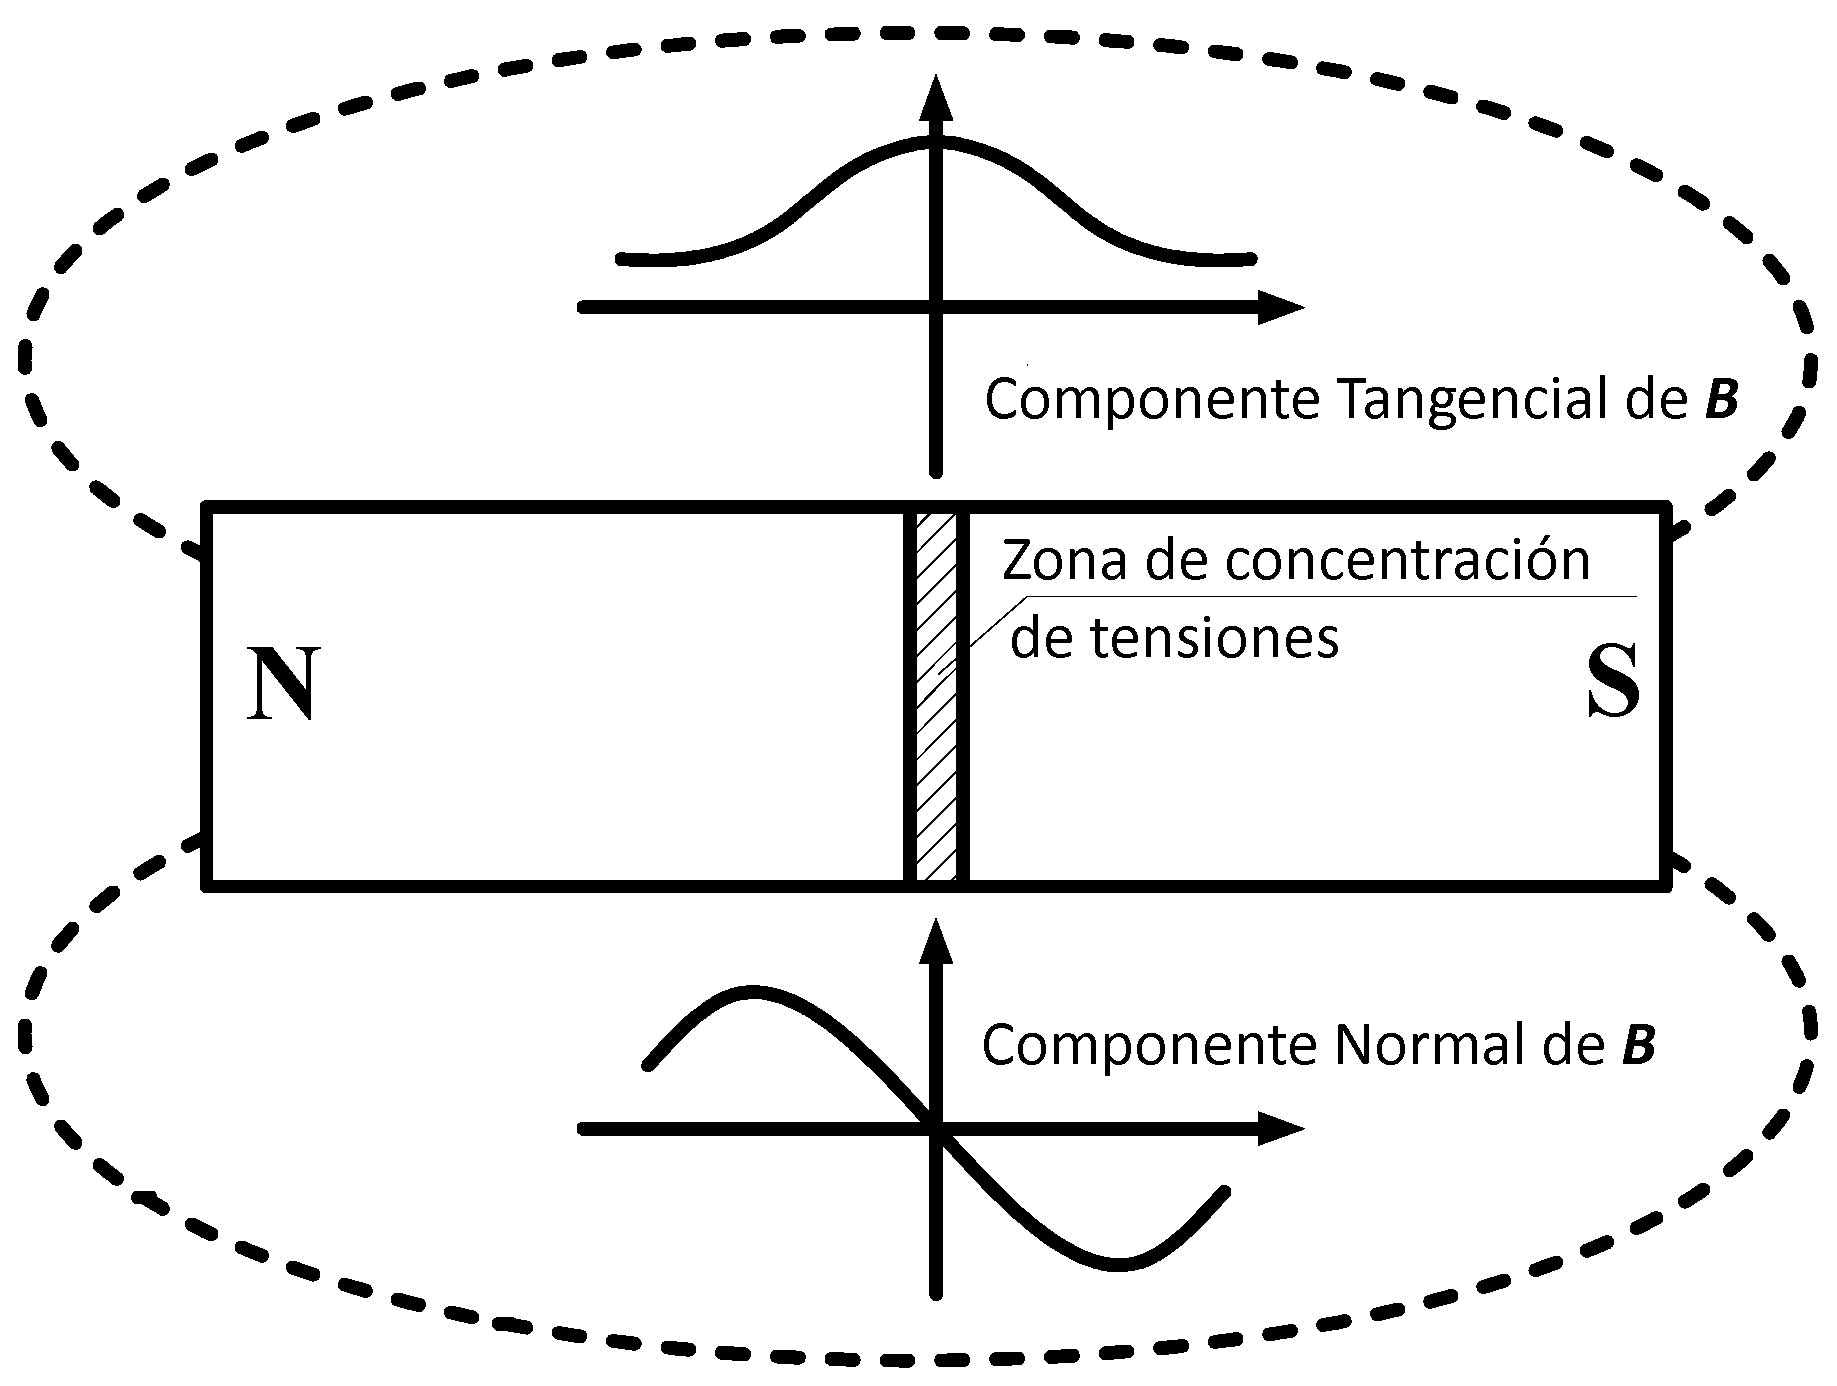
\includegraphics[width=0.75\textwidth]{./Figures/metals-09-00661-g001.jpg}
	\caption{Componentes del campo $B$ asociadas a perturbaciones debidas a heterogeneidades magnéticas primarias\protect\footnotemark.}
	\label{fig:metals-09-00661-g001}
\end{figure}
\footnotetext{\url{https://www.mdpi.com/2075-4701/9/6/661}}

La medición de las no uniformidades de la magnetización permite detectar los defectos en forma no destructiva. 
En general no es posible obtener información en forma global del campo magnético autogenerado en sólidos. La información se forma y se puede obtener solo en pequeñas regiones donde los defectos tienen una influencia significativa por su cercanía y no se ven afectados por otros defectos. Es de esperarse que en los defectos significativos, el campo externo de la tierra no haya podido ejercer una influencia marcada si la energía asociada a la producción del defecto es muy superior a la aportada por el campo magnético externo.

El método MMM se aplica para la solución de problemas del tipo de:


\begin{itemize}
	\item Control de calidad al 100\verb|%| de piezas súper críticas de construcción de máquinas y control de heterogeneidad del metal. 
	\item Control de calidad de juntas de soldadura (Aquí la soldadura es parte de un complejo sistema de factores vinculando la: heterogeneidad estructural-mecánica, los defectos de soldadura y las  concentraciones de estrés estructural. 
	\item Diagnóstico temprano de daños por fatiga del metal. Estimación y pronóstico del tiempo de vida media de un componente mecánico.
\end{itemize}


El MMM se puede aplicar tanto en sólidos bajo carga (en tensión como en el caso de piezas de maquinaria) así como después del retiro de las cargas cuando la pieza no se encuentra solicitada. El perfil magnético formado bajo la acción de las cargas de trabajo queda parcialmente congelado después de la descarga en virtud de la histéresis de dislocación magnética\citep{Dislocaciones}. Esto da la posibilidad de evaluar el estado real de tensiones de la pieza y revelar en etapas tempranas las zonas de daño máximo al leer los campos utilizando dispositivos de medición de características especiales. Es importante destacar que los dispositivos de medición de campos magnéticos no tienen una norma mundial por lo que cada instrumento presenta características y singularidades únicas y las mediciones no suelen ser referidas a un patrón sino que son relativas entre sí desde un estado base.

\subsection{El MMM y los sólidos ferromagnéticos.}

Los sólidos ferromagnéticos en presencia del campo magnético terrestre, presentan una magnetización inducida fuertemente perfilada por las condiciones de frontera magnética. El campo inducido divergirá en las zonas de discontinuidad superficial del material y en zonas de \textit{stress}, oquedades o inclusiones de otros materiales en el seno del material original. 
Cuando un sólido ferromagnético se enfría por debajo de su temperatura de Curie el campo magnético terrestre genera un patrón de dominios. Posteriormente, cuando el material se trabaja, asociado a los procesos térmicos o por deformación en frío se producen defectos en la estructura policristalina y eventualmente algunos defectos estructurales presentarán concentraciones de esfuerzos y deformaciones importantes. Estas concentraciones alteran localmente los dominios magnéticos y producen a su vez, heterogeneidades en la magnetización que pueden ser detectadas midiendo la dispersión del campo magnético en la superficie de los cuerpos. 
Para estos sólidos es particularmente útil el MMM. 

El método también puede aplicarse, con menor grado de facilidad, a materiales  antiferromagnéticos, ferrimagnéticos y paramagnéticos.


%Los detalles los podemos encontrar en el apéndice \ref{AppendixLaminacionYTrenes}


